\documentclass[11pt]{article}
\usepackage{colacl}
\usepackage{graphicx}
\usepackage{float}
\sloppy
\raggedbottom
\setlength\titlebox{1.2in}
\makeatletter
\renewcommand\section{%
    \@startsection{section}{1}{\z@}%
                  {-2.4ex plus -0.6ex minus -0.3ex}%
                  {1.0ex plus 0.3ex minus 0.2ex}%
                  {\large\bf\raggedright}}
\renewcommand\subsection{%
    \@startsection{subsection}{2}{\z@}%
                  {-1.8ex plus -0.4ex minus -0.2ex}%
                  {0.75ex plus 0.2ex minus 0.1ex}%
                  {\normalsize\bf\raggedright}}
\makeatother



\title{COMP30027 Report}




\begin{document}
\maketitle


%\begin{abstract}
%Don't include an abstract.
%\end{abstract}

\section{Introduction}
This project studies supervised image classification under a coarse-to-fine setting.
Task 1 is a coarse-grained animal classification problem, where the target classes
belong to visually distinct animal categories. Task 2 is a fine-grained bird species
classification problem, where the classes are more visually similar and often differ
only in subtle colour, texture, shape, or local markings. The contrast between these
two tasks makes it possible to examine how feature representations and classifiers
behave as the classification problem becomes more fine-grained.

In this report, I compare provided hand-crafted image descriptors, including colour
histograms, HOG, and additional low-level features, with learned representations
extracted from ImageNet-pretrained convolutional neural networks. I then evaluate
several classifiers on both tasks using accuracy and macro-F1, analyse the main
performance differences, and discuss the errors and limitations revealed by the
coarse-to-fine progression.



\section{Methodology}

\subsection{Feature Representations}
For both tasks, I first used the provided hand-crafted image descriptors,
including colour histograms, HOG descriptors, and additional 
low-level image statistics. These representations capture colour distribution, 
edge orientation, texture variation, and simple global image properties.
They provide interpretable baselines, although they may be limited for fine-grained
recognition where class differences are subtle and local. HOG descriptors were
included because edge orientation is a useful cue for shape and local
structure~\cite{dalal2005histograms}.

I also used ImageNet-pretrained convolutional neural networks as fixed feature extractors. 
In this approach, each image is passed through a pretrained CNN, and the final classification layer 
is removed so that the network output is used as a deep embedding. 
I experimented with \textbf{ResNet} and \textbf{EfficientNet} variants, with EfficientNet-V2-L giving the strongest representation in later experiments. 
These CNN outputs were treated as engineered feature representations rather than
end-to-end neural classifiers, so they could be concatenated with the provided
features and passed to the same set of supervised learners.
The CNNs were not fine-tuned on the project data, CIFAR-10, or CUB-200-2011; 
they were used only as generic ImageNet-pretrained feature extractors, which satisfies the project constraints~\cite{deng2009imagenet,tan2021efficientnetv2}.


\subsection{Classifiers}
I evaluated linear, non-linear, probabilistic, distance-based, and ensemble
classifiers. Logistic Regression and Linear SVM tested whether the learned feature
space was approximately linearly separable, while RBF SVM allowed curved decision
boundaries~\cite{cortes1995support}. I also evaluated KNN, Gaussian Naive Bayes,
Random Forest, and Extra Trees; the tree ensembles can capture non-linear feature
interactions~\cite{breiman2001random,geurts2006extremely}.

\subsection{Evaluation Protocol}
For model evaluation, I used stratified train-validation splits for the main result tables 
and error analysis, and 5-fold stratified cross-validation during hyperparameter screening. 
Thus, the validation results reported in the tables refer to the held-out validation split 
unless explicitly described as cross-validation. Stratification was used to preserve the 
class distribution in each split, which is important for both 10-class classification tasks. 
Accuracy was the primary metric because the Kaggle competitions evaluate submissions using classification accuracy. 
Macro-F1 was also reported to check whether performance was balanced across all classes rather than dominated by easier categories.

Hyperparameters were selected using only the labelled training data, including
regularisation strength, preprocessing strategy, SVM kernel parameters, and tree
ensemble settings.
After selecting the best configuration, the final model was retrained on the full labelled training set before generating Kaggle predictions for the unlabelled test images.


\section{Results}

\subsection{Task 1: Coarse-Grained Classification}
Table~\ref{tab:task1-results} summarises the main Task 1 validation results. 
Using only the provided hand-crafted descriptors gave relatively weak performance, 
with the best baseline accuracy around 54.4\%. Adding ImageNet-pretrained 
CNN embeddings substantially improved performance. The best Task 1 validation 
result was obtained using colour, HOG, additional features, and EfficientNet-V2-L embeddings, 
reaching 97.3\% accuracy and 97.3\% macro-F1 with Logistic Regression. This suggests that 
the pretrained CNN representation captured more discriminative visual structure than simple hand-crafted features alone.

\begin{table}[h]
\centering
\small
\begin{tabular}{p{0.48\linewidth}cc}
\hline
Features & Accuracy & Macro-F1 \\
\hline
Colour + HOG + additional & 0.544 & 0.541 \\
HOG + additional + EffNet-V2-M & 0.931 & 0.931 \\
Colour + HOG + additional + EffNet-V2-L & 0.973 & 0.973 \\
\hline
\end{tabular}
\caption{Selected Task 1 held-out validation results. EffNet denotes EfficientNet.}
\label{tab:task1-results}
\end{table}

After selecting the strongest Task 1 representation, I compared several classifiers 
on the same colour, HOG, additional features, and EfficientNet-V2-L feature set. 
Table~\ref{tab:task1-models} shows a small comparison across linear, kernel-based, 
and ensemble models.

\begin{table}[h]
\centering
\small
\begin{tabular}{lcc}
\hline
Model & Accuracy & Macro-F1 \\
\hline
Logistic Regression & 0.973 & 0.973 \\
RBF SVM & 0.963 & 0.963 \\
Random Forest & 0.957 & 0.957 \\
\hline
\end{tabular}
\caption{Selected Task 1 held-out validation comparison of models using colour, HOG, additional features, and EfficientNet-V2-L embeddings.}
\label{tab:task1-models}
\end{table}

Logistic Regression performed best, while RBF SVM and Random Forest were close. 
This suggests that the EfficientNet-V2-L representation made Task 1 largely separable 
without requiring a more complex classifier.


\subsection{Task 2: Fine-Grained Classification}
Task 2 was more challenging than Task 1 because the classes are visually 
similar bird species and the labelled training set is much smaller. 
Initial experiments using the provided low-level descriptors gave limited performance compared 
with later combinations that included CNN embeddings. The strongest representation combined 
HOG, additional features, and EfficientNet-V2-L embeddings, and this feature set gave 
consistently strong performance across different classifiers.

Table~\ref{tab:task2-validation} reports the main Task 2 results for this 
strongest representation. Tree-based ensemble models achieved the strongest performance, 
with Random Forest and Extra Trees obtaining the highest accuracy among the evaluated 
classifiers. Logistic Regression and RBF SVM also performed strongly, 
which suggests that the EfficientNet-V2-L embedding made the bird species substantially 
more separable than the hand-crafted descriptors alone. The relatively small gap between 
the best models also indicates that the representation itself was more important than the choice of classifier.


\begin{table}[h]
\centering
\footnotesize
\begin{tabular}{lccc}
\hline
Model & Accuracy & Macro-F1 & Notes \\
\hline
Random Forest & 0.976 & 0.975 & Ensemble \\
Extra Trees & 0.976 & 0.975 & Ensemble \\
Logistic Reg. & 0.952 & 0.951 & Linear \\
RBF SVM & 0.952 & 0.951 & Kernel \\
Linear SVM & 0.952 & 0.951 & Linear \\
KNN & 0.940 & 0.939 & Distance \\
Gaussian NB & 0.940 & 0.938 & Probabilistic \\
\hline
\end{tabular}
\caption{Task 2 held-out validation results using HOG, additional features, and EfficientNet-V2-L embeddings.}
\label{tab:task2-validation}
\end{table}

\subsection{Cross-Task Comparison}
Across both tasks, the strongest results came from combining selected provided
descriptors with ImageNet-pretrained CNN embeddings. The final feature choices
also reflected the coarse-to-fine setting. Colour was kept for Task 1 because
coarse animal categories often differ in global colour and overall appearance.
For Task 2, the global colour histogram was not included in the final feature set
because bird species can have highly overlapping colour distributions; it was
therefore more likely to be redundant or noisy than HOG, additional features, and
EfficientNet-V2-L representations, which better encode shape, texture, and local
visual evidence. Once EfficientNet-V2-L embeddings were included, several
classifiers achieved similar validation performance, indicating that the main
gain came from improving the representation rather than only choosing a more
complex classifier.



\section{Discussion and Critical Analysis}

\subsection{Effect of Feature Representations}
The main finding is that the choice of representation had a larger effect than
the choice of classifier. The provided descriptors were useful baselines because
they encode interpretable low-level properties such as colour distribution, edge
orientation, texture, and simple image statistics. However, these features do not
fully capture invariance to pose, viewpoint, scale, and background variation. This
explains why they were not sufficient on their own, especially for Task 2.

Pretrained CNN embeddings improved both tasks because they provide a hierarchical
visual representation learned from a much larger image collection~\cite{deng2009imagenet,yosinski2014transferable}. 
Earlier layers capture local edges and textures, while later layers represent more 
abstract object parts and shapes~\cite{zeiler2014visualizing}. This is useful for 
Task 1 because animal categories can often be separated by broad shape and appearance 
cues. It is even more important for Task 2, where the relevant evidence may be a small 
local cue such as a bill marking, head colour, or wing pattern. In this sense, the CNN 
features reduce the burden placed on the classifier: after the image has been mapped 
into a stronger feature space, even relatively simple models can separate many classes well.

The improvement from EfficientNet-V2-M to EfficientNet-V2-L suggests that
representation capacity also mattered. The larger model likely captured richer
visual patterns that transferred better to fine-grained bird recognition. At the
same time, the CNNs were used only as fixed ImageNet-pretrained feature extractors,
not fine-tuned on CUB-200-2011 or the project data. Therefore, the performance gain
should be interpreted as the benefit of transfer learning rather than supervised
adaptation to the target classes.

\subsection{Effect of Classifier Choice}
Classifier choice still mattered, but its effect was smaller once strong CNN
embeddings were included. Logistic Regression and Linear SVM performed well,
which suggests that EfficientNet-V2-L made many classes close to linearly
separable. RBF SVM did not give a large improvement over the linear models, which
again indicates that much of the useful non-linearity had already been introduced
by the CNN feature extractor.

This connects to the bias-variance trade-off discussed in lectures. With a
high-dimensional but informative representation, a lower-variance linear model can
generalise well from a small labelled dataset. More flexible models can capture
non-linear interactions, but they also have more scope to fit validation-specific
patterns. This also matches the lecture view of CNNs as neural networks that learn
increasingly abstract features: the CNN performs the non-linear feature learning,
while the final classifier only needs a simpler decision boundary.

The relative behaviour of Random Forest also differed across the two tasks. In
Task 1, Logistic Regression was slightly stronger than Random Forest, suggesting
that the coarse animal classes were already well separated in the EfficientNet
feature space. In Task 2, Random Forest and Extra Trees achieved the best
validation results, suggesting that fine-grained bird recognition benefited more
from non-linear interactions between CNN dimensions and low-level descriptors. This
conclusion should still be treated cautiously because the Task 2 validation split
contains only 84 images; a difference of one or two predictions can noticeably
change the reported accuracy.
Overall, Task 1 favoured simpler linear classifiers once strong CNN features were
available, whereas Task 2 benefited more from ensemble methods because the
fine-grained bird classes required subtler non-linear feature interactions.

\subsection{Error Analysis}
The aggregate metrics suggest that Task 1 errors were relatively limited: the best
Task 1 model reached 97.3\% accuracy and 97.3\% macro-F1. Because accuracy and
macro-F1 were almost identical, the remaining mistakes were unlikely to be
concentrated in one or two weak classes. This is consistent with the
coarse-grained setting, where broad shape and appearance cues separate most animal
categories. By contrast, Task 2 provides a clearer view of the remaining weakness
of the approach because its classes are visually closer.

The Task 2 validation errors were concentrated in a small number of visually
similar pairs. Using the HOG, additional features, and EfficientNet-V2-L
representation, both Random Forest and Extra Trees made two errors on the 84-image
validation split. In both models, one Ring-billed Gull image was predicted as
Herring Gull, and one Yellow Warbler image was predicted as Wilson Warbler, as
shown for Random Forest in Figure~\ref{fig:task2-confusion-matrix}. The
corresponding recalls were 7/8 for Ring-billed Gull and 7/8 for Yellow Warbler,
while all other classes had perfect recall in these two models.

\begin{figure}[t]
\centering
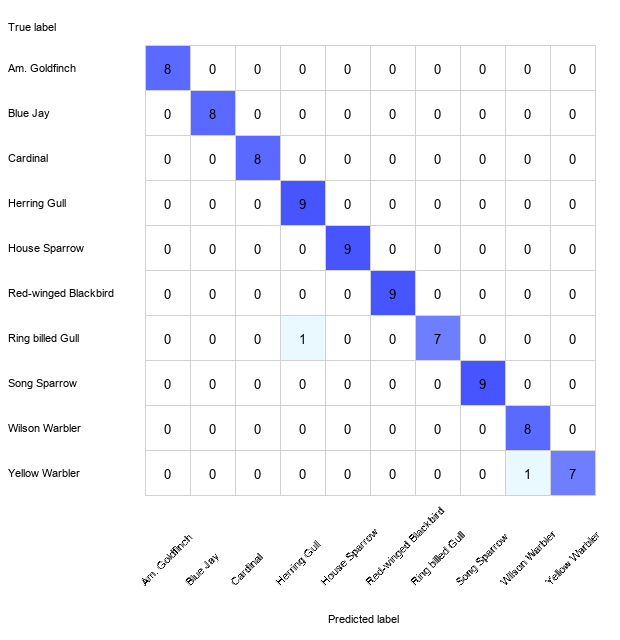
\includegraphics[width=0.94\linewidth]{../outputs/figures/task2_random_forest_confusion_matrix.png}
\caption{Task 2 validation confusion matrix for Random Forest using HOG, additional features, and EfficientNet-V2-L embeddings.}
\label{fig:task2-confusion-matrix}
\end{figure}

These errors are meaningful because they are not random confusions between
unrelated species. Herring Gull and Ring-billed Gull share a similar white and grey
body structure, so the distinction depends on subtle bill markings. Yellow Warbler
and Wilson Warbler are also visually close because both are small yellow birds, and
the distinguishing black cap of the Wilson Warbler may be hard to detect when the
head region is small or poorly positioned. The absence of errors between visually
distinctive species suggests that the model learned broad colour and shape cues,
but still struggled when the decision depended on a small local visual cue.

\subsection{Coarse-to-Fine Reflection}
The coarse-to-fine progression reveals both the strength and limitation of the
current approach. Transfer learning provides a strong general visual representation
even when the labelled dataset is small, explaining why the same EfficientNet-based
strategy worked well on both tasks. However, whole-image features are less ideal
when the decision depends on a small discriminative part. Fine-grained
classification therefore exposes a gap between recognising the general object type
and localising the evidence needed to separate similar species.


\subsection{Limitations}
One limitation is that the pretrained CNNs were fixed feature extractors, so the
representation was not adapted to the target bird species. The pipeline also did
not perform object localisation, part detection, or region-of-interest modelling.
Fine-grained recognition often benefits from focusing on the head, wing, or bill,
but whole-image summaries may dilute these small cues~\cite{zhang2014part}.

The small size of the Task 2 training set also makes model selection less stable.
Although stratified cross-validation reduces dependence on a single split, the
validation folds are still small. Therefore, small differences between the top
models should not be over-interpreted. This is why I considered both accuracy and
macro-F1 and compared several model families.


\section{Conclusion}
This project showed that image representation was the most important factor in both coarse-grained and fine-grained classification. 
The provided low-level descriptors were useful as baseline features, but the strongest results came from combining selected provided 
descriptors with ImageNet-pretrained CNN embeddings.
In particular, the final models used EfficientNet-V2-L with HOG and additional features, plus colour for Task 1.

The coarse-to-fine comparison showed that fine-grained bird classification requires richer representations 
because the classes differ in subtle local details rather than broad visual categories. 
Once strong CNN embeddings were used, several classifiers achieved high accuracy, suggesting 
that the representation made the classes substantially more separable. Overall, the results 
support the value of transfer learning for small image classification datasets, while also 
showing the limitations of whole-image features for fine-grained recognition.

\bibliographystyle{acl}
\bibliography{sample}

\end{document}
